%____________________________________________________________________________||
\section{Event selection and categorisation}
\label{app:selection}

\begin{figure}[h!]
    \begin{center}
        {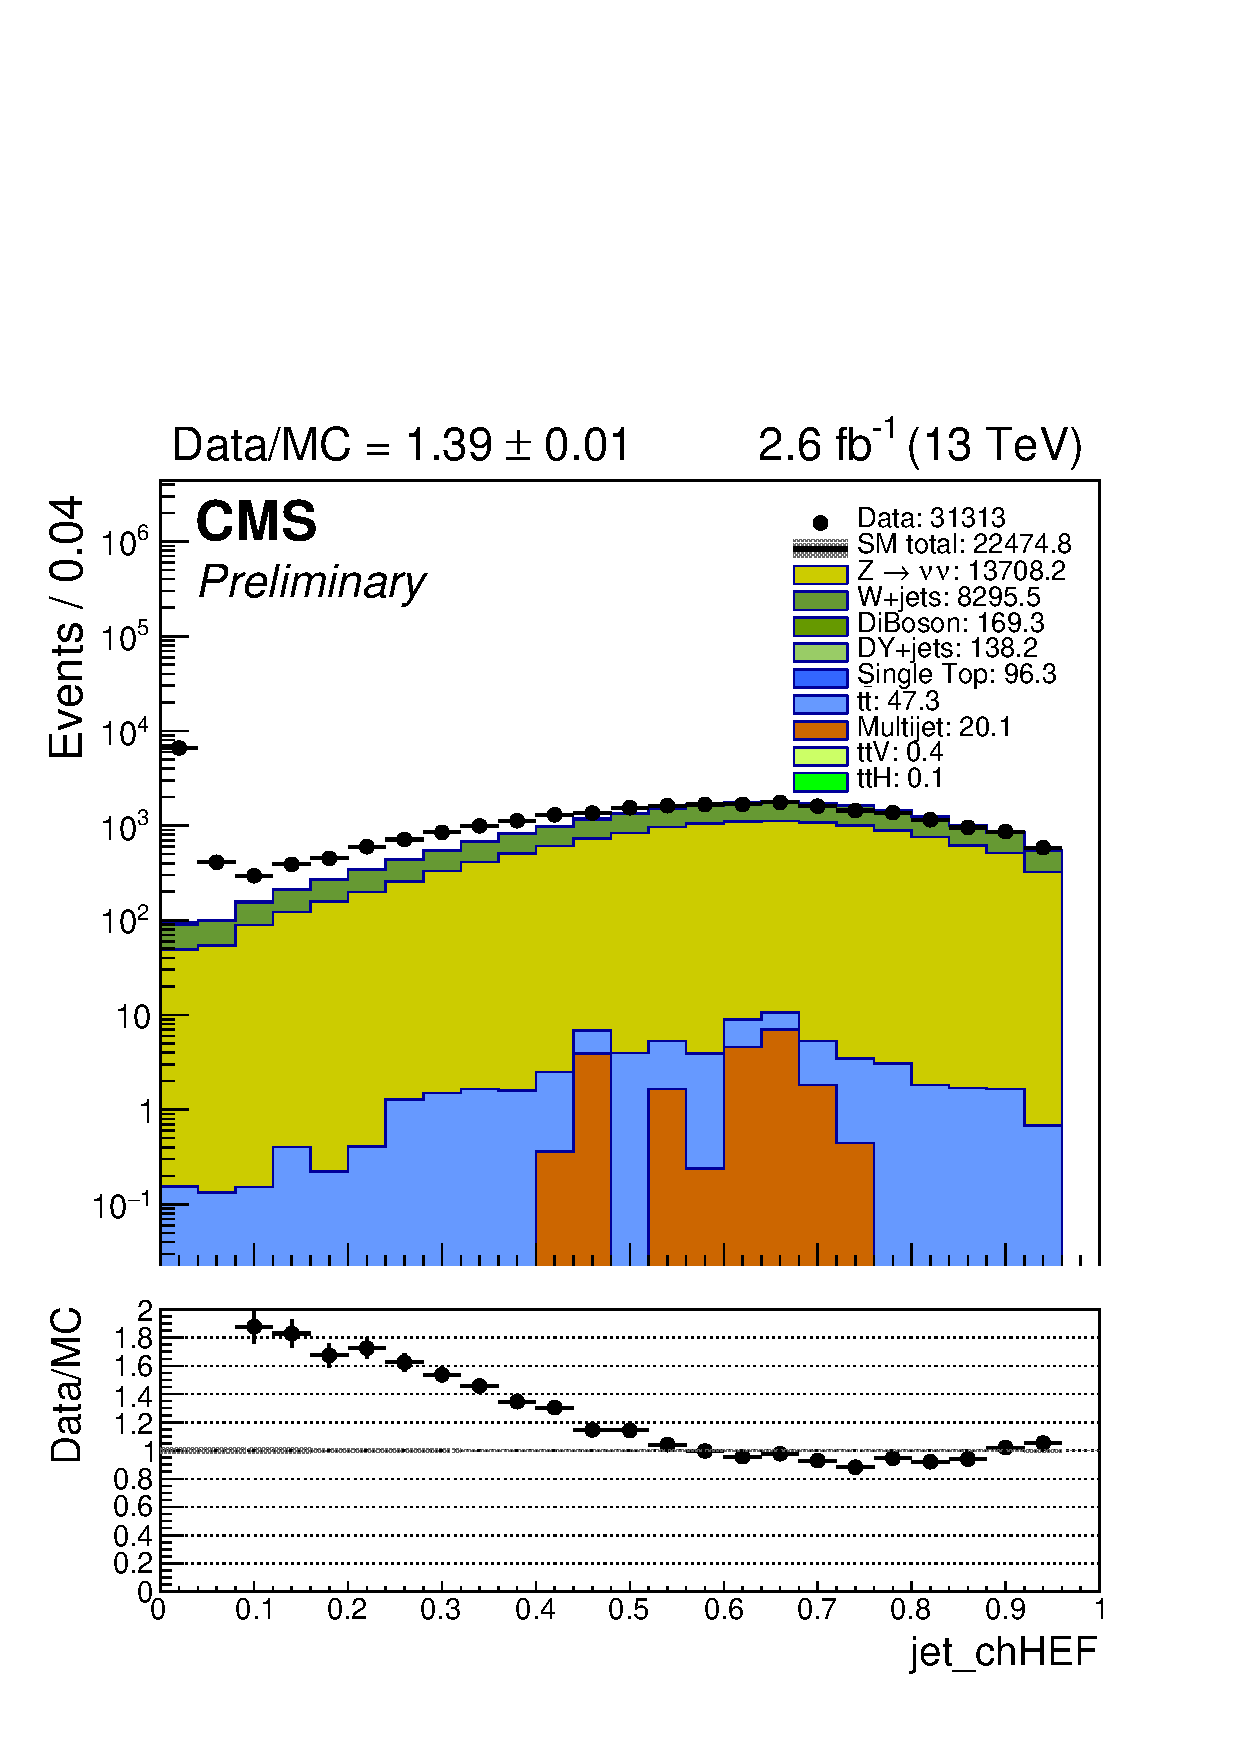
\includegraphics[width=0.32\textwidth]{figures/selection/jet_chHEF_mono_all_before.pdf}}
        {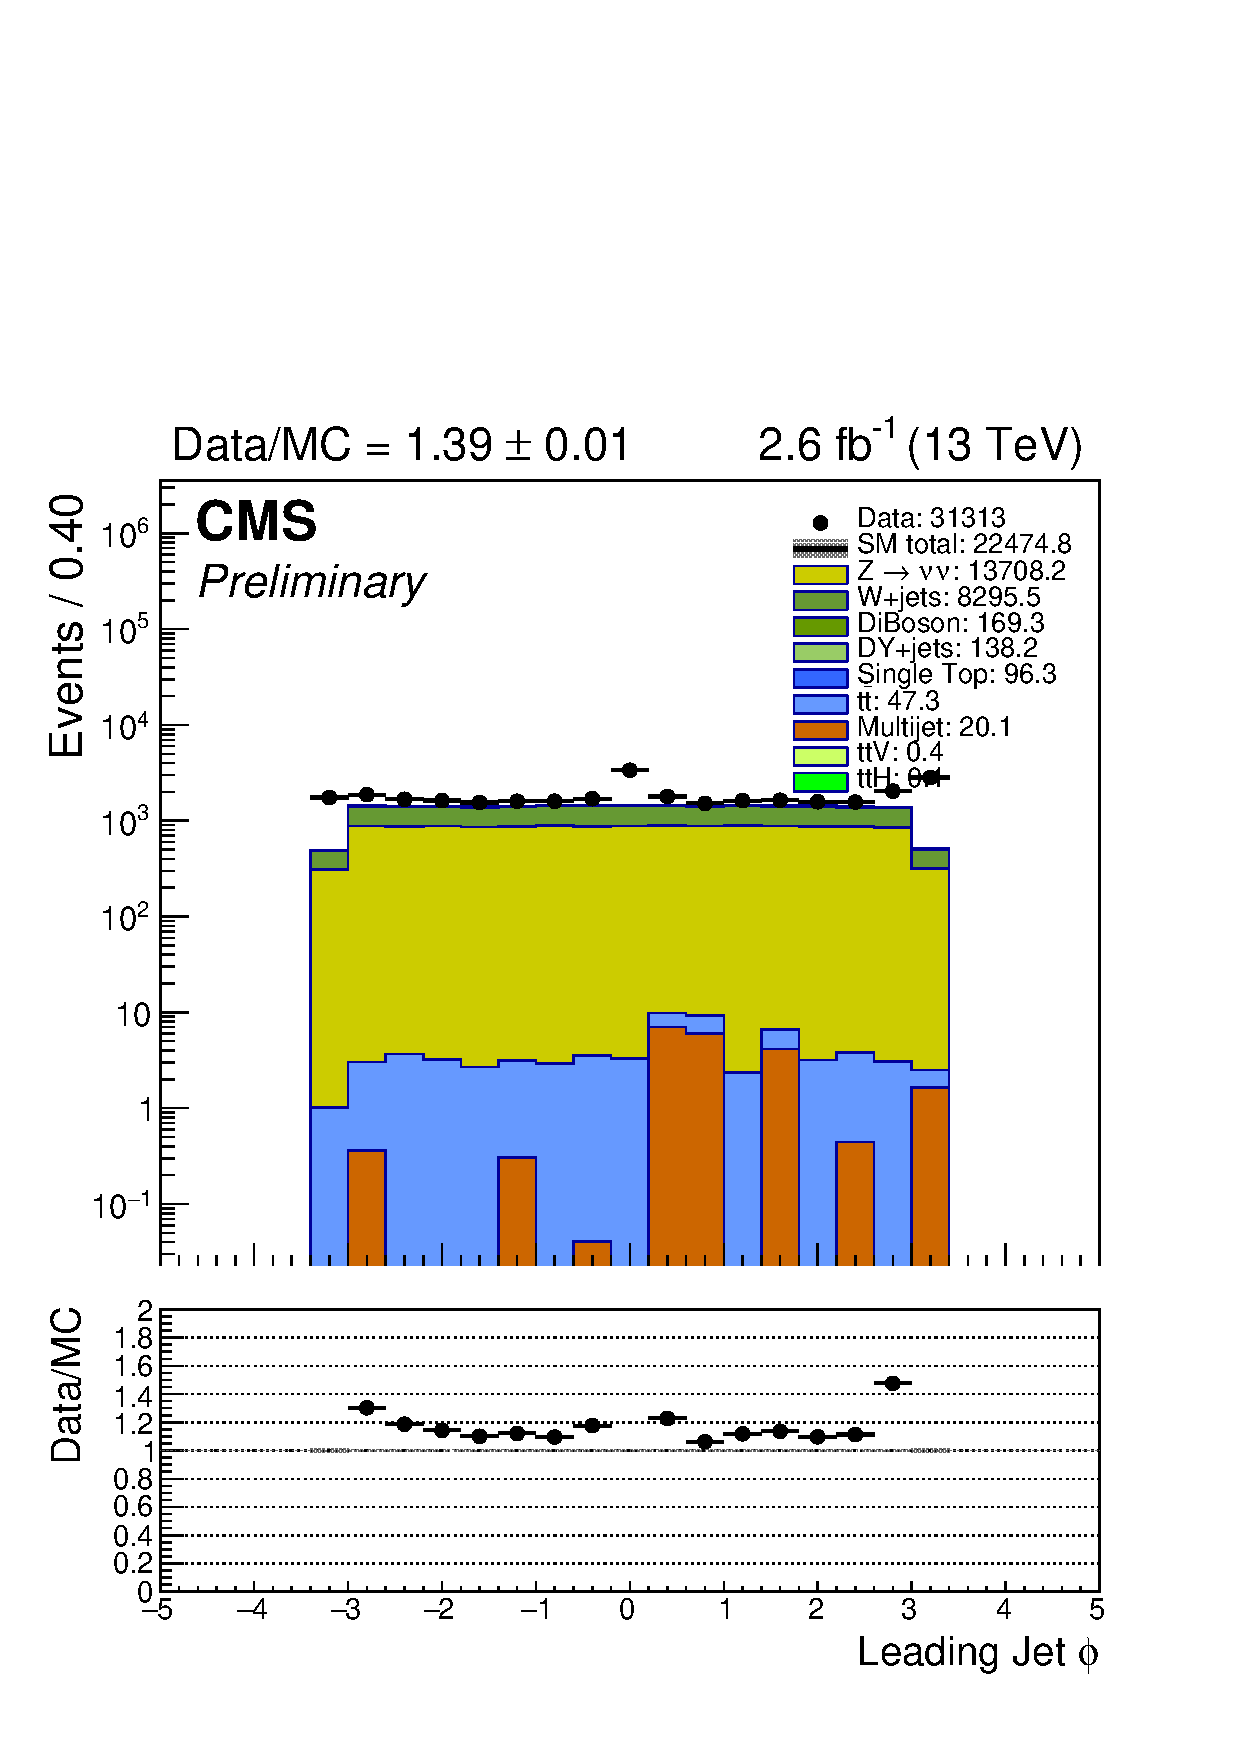
\includegraphics[width=0.32\textwidth]{figures/selection/jet_phi[0]_mono_all_before.pdf}}
        {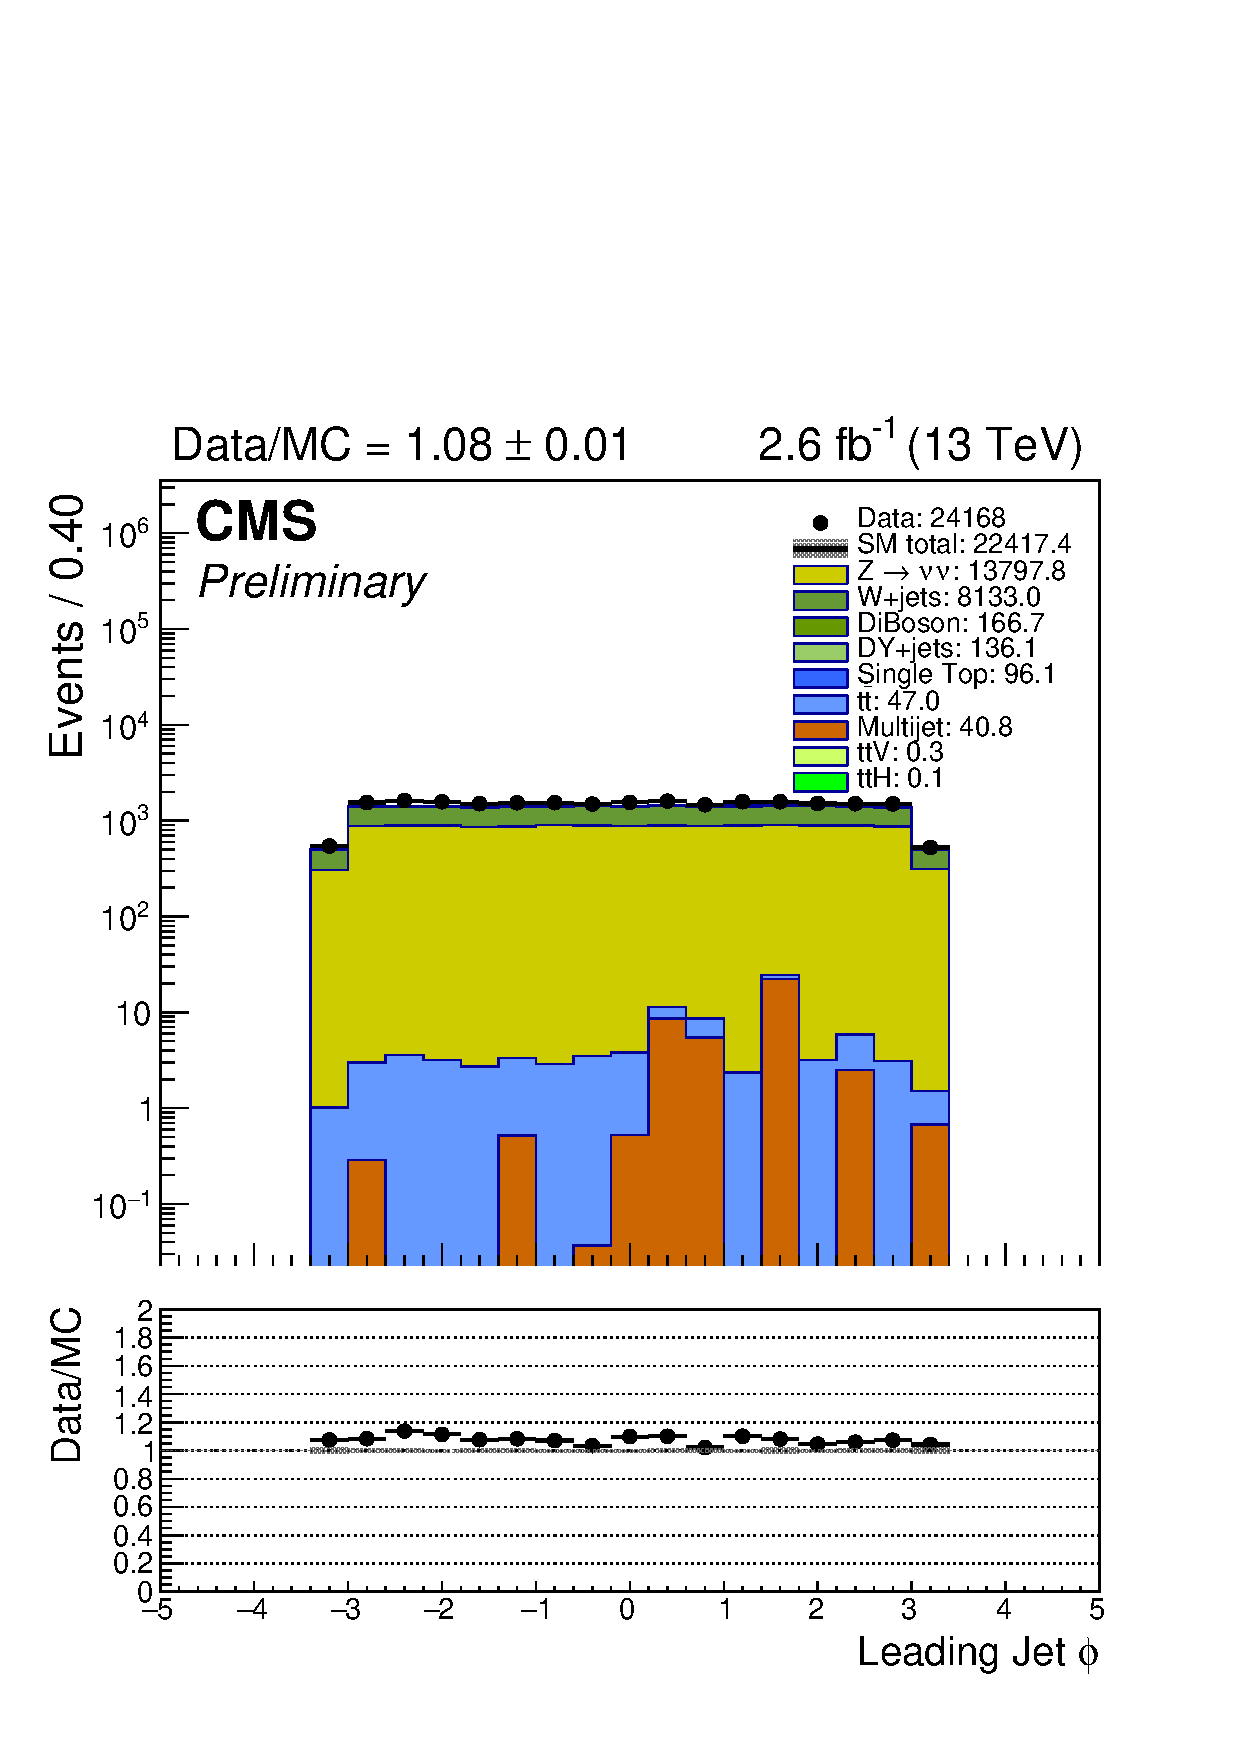
\includegraphics[width=0.32\textwidth]{figures/selection/jet_phi[0]_mono_all_after.pdf}}
        \caption{Distributions in the signal region of (Left) the jet
          charged hadron energy fraction (CHF), (Centre) the jet
          $\phi$ direction, and (Right) jet $\phi$ direction after
          applying a requirement of {CHF~$>0.1$}. The large excess in
          data at charged hadron fractions close to zero and ${\phi =
            0, \pi}$ is consistent with beam halo effects, and is
          effectively suppressed by the aforementioned selection.}
        \label{fig:leadJetCleaning}
    \end{center}
\end{figure}

\begin{figure}[h!]
  \begin{center}
    {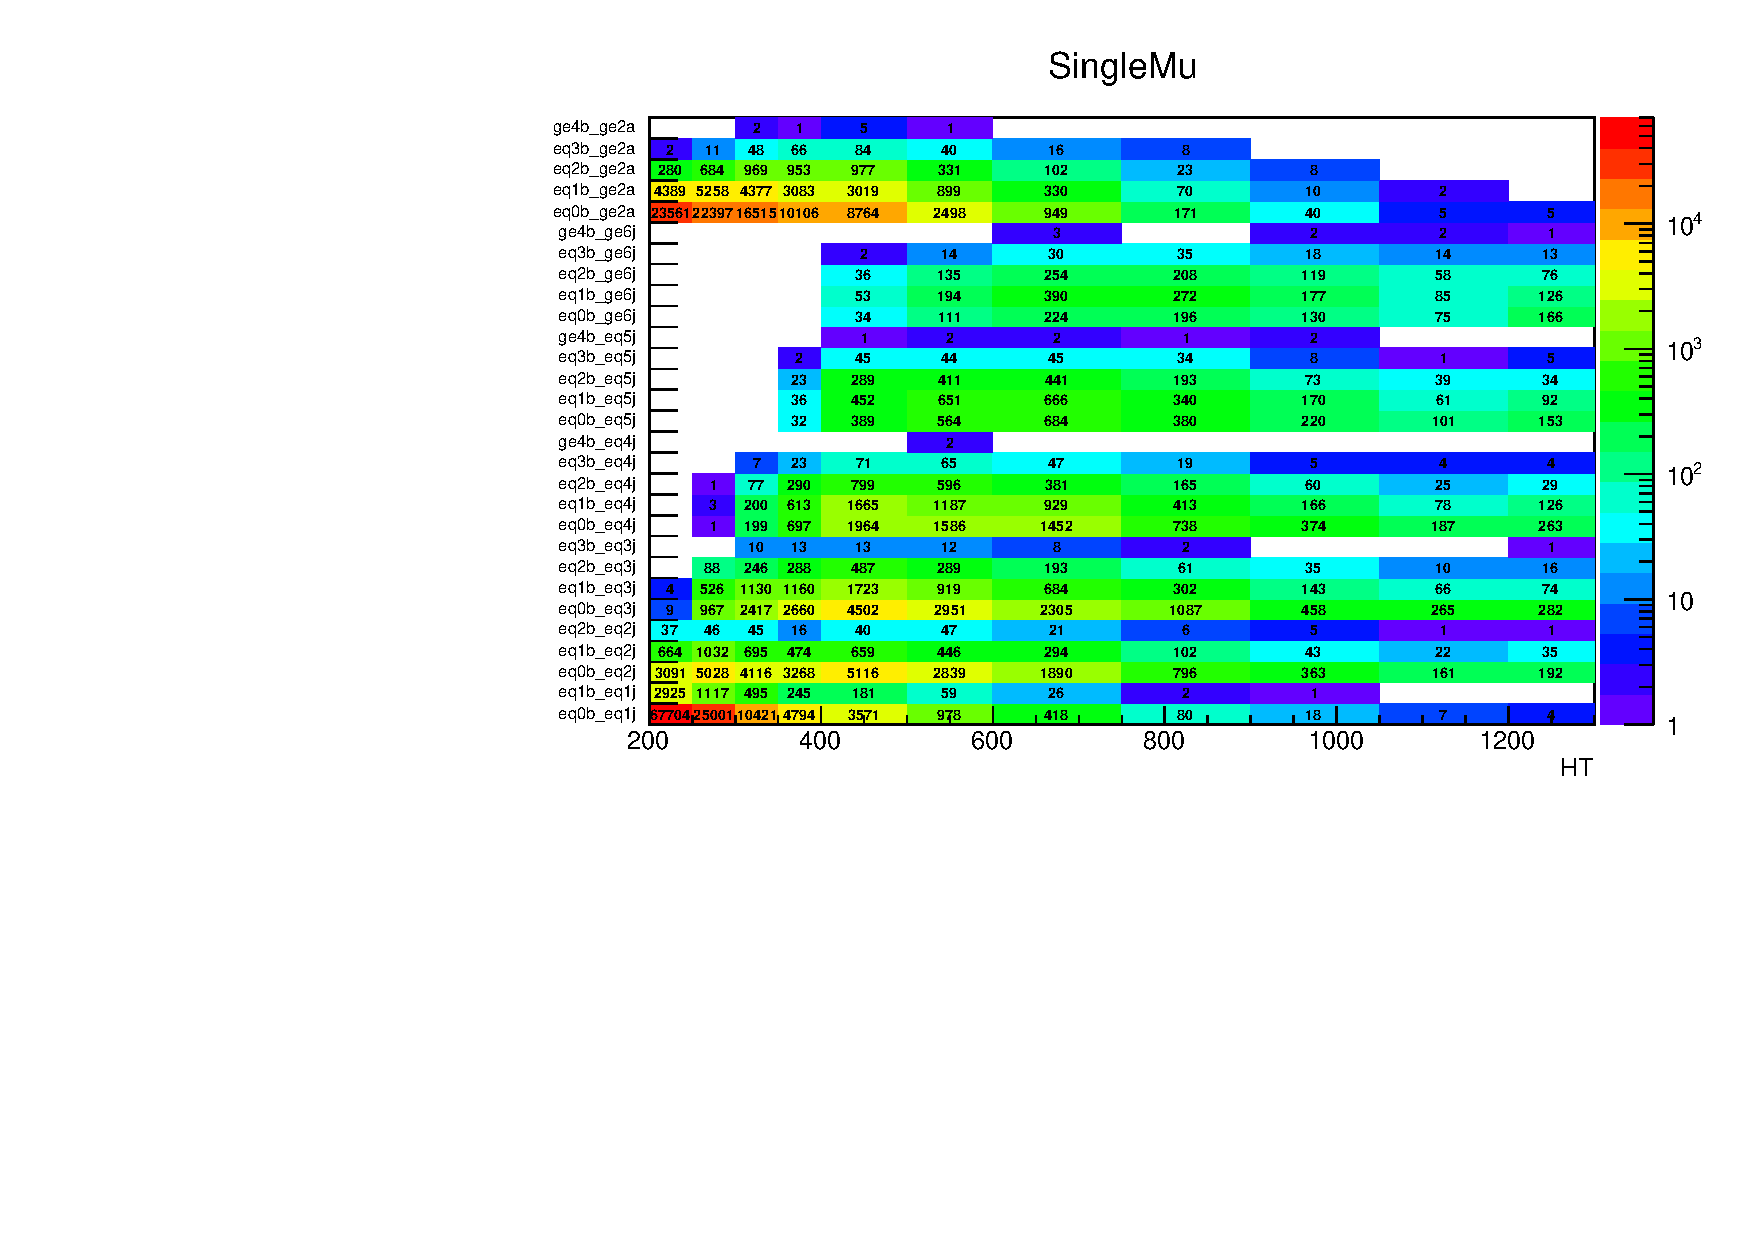
\includegraphics[width=0.6\textwidth]{figures/control_regions/SingleMu.pdf}} 
    {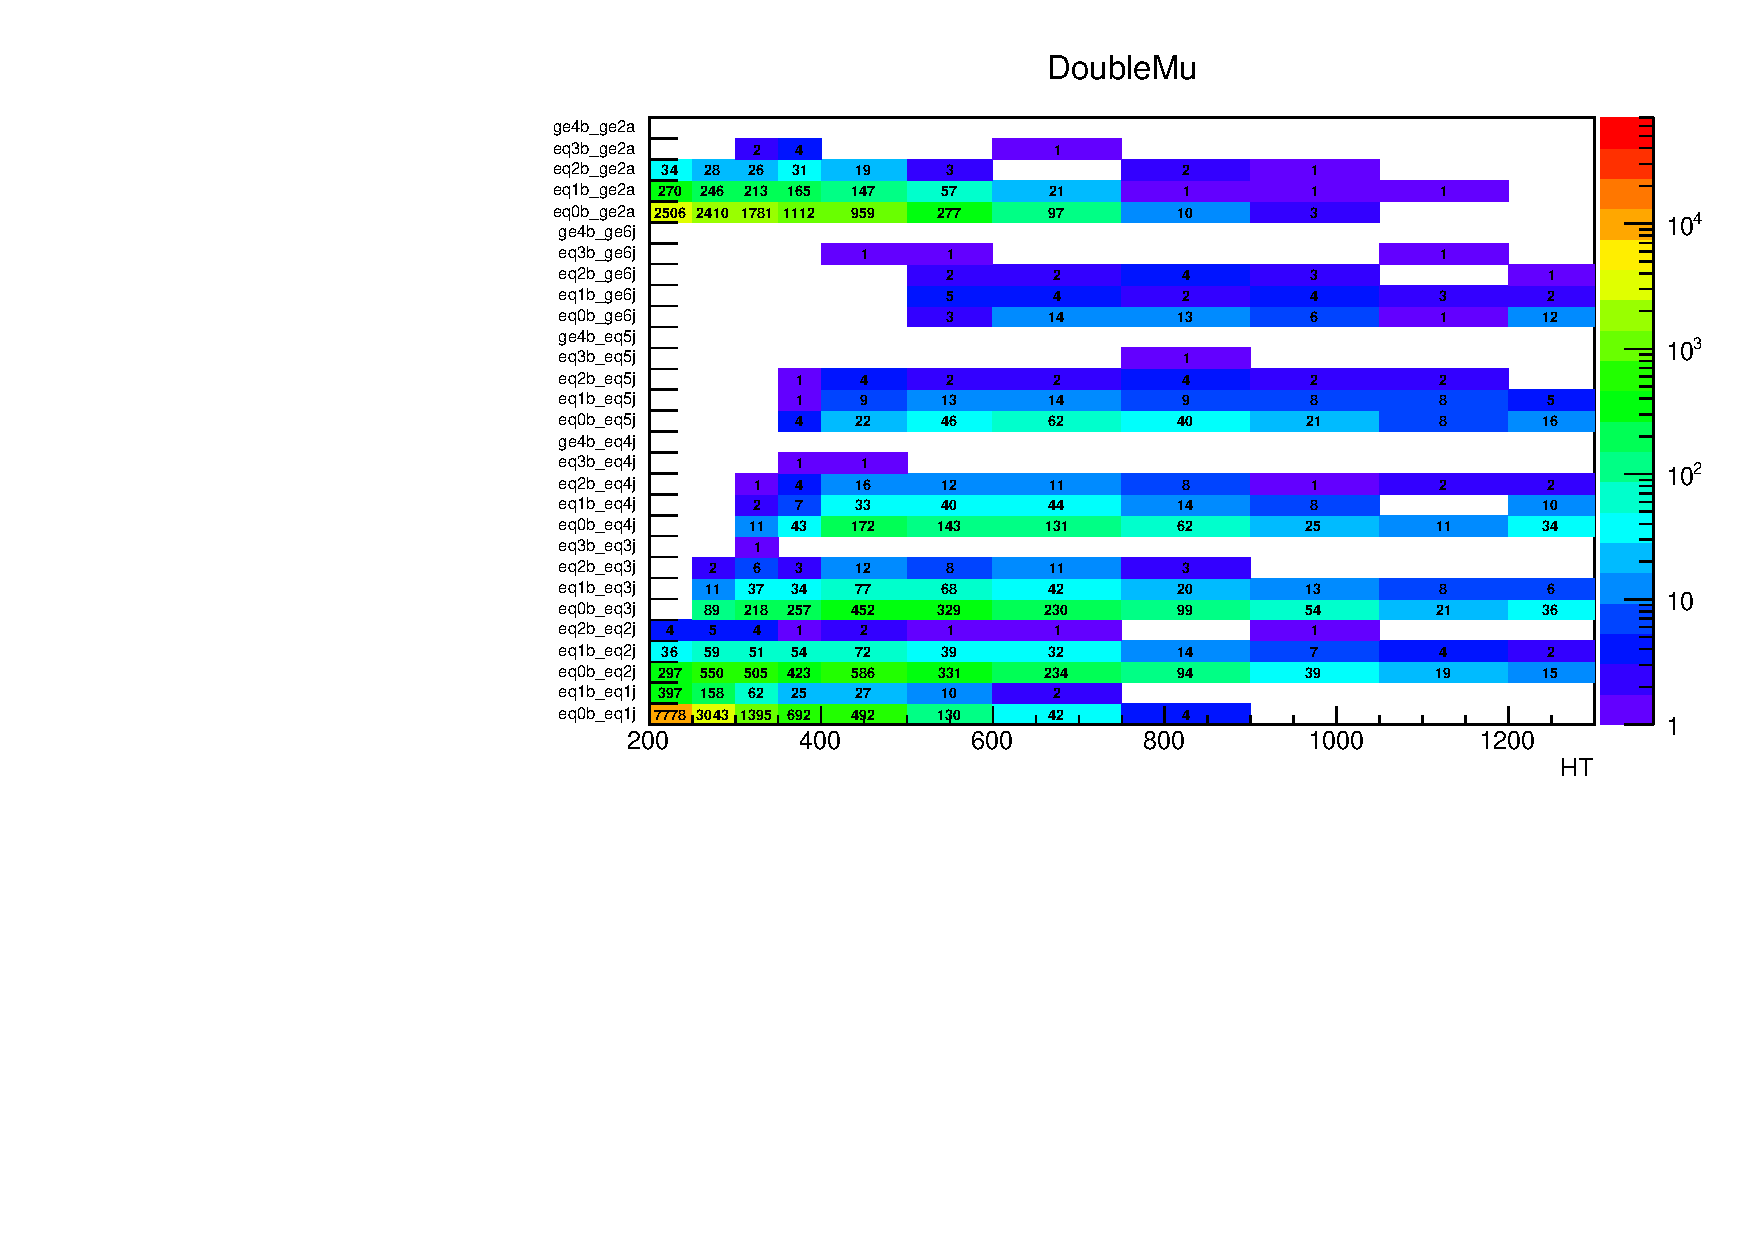
\includegraphics[width=0.6\textwidth]{figures/control_regions/DoubleMu.pdf}}
    {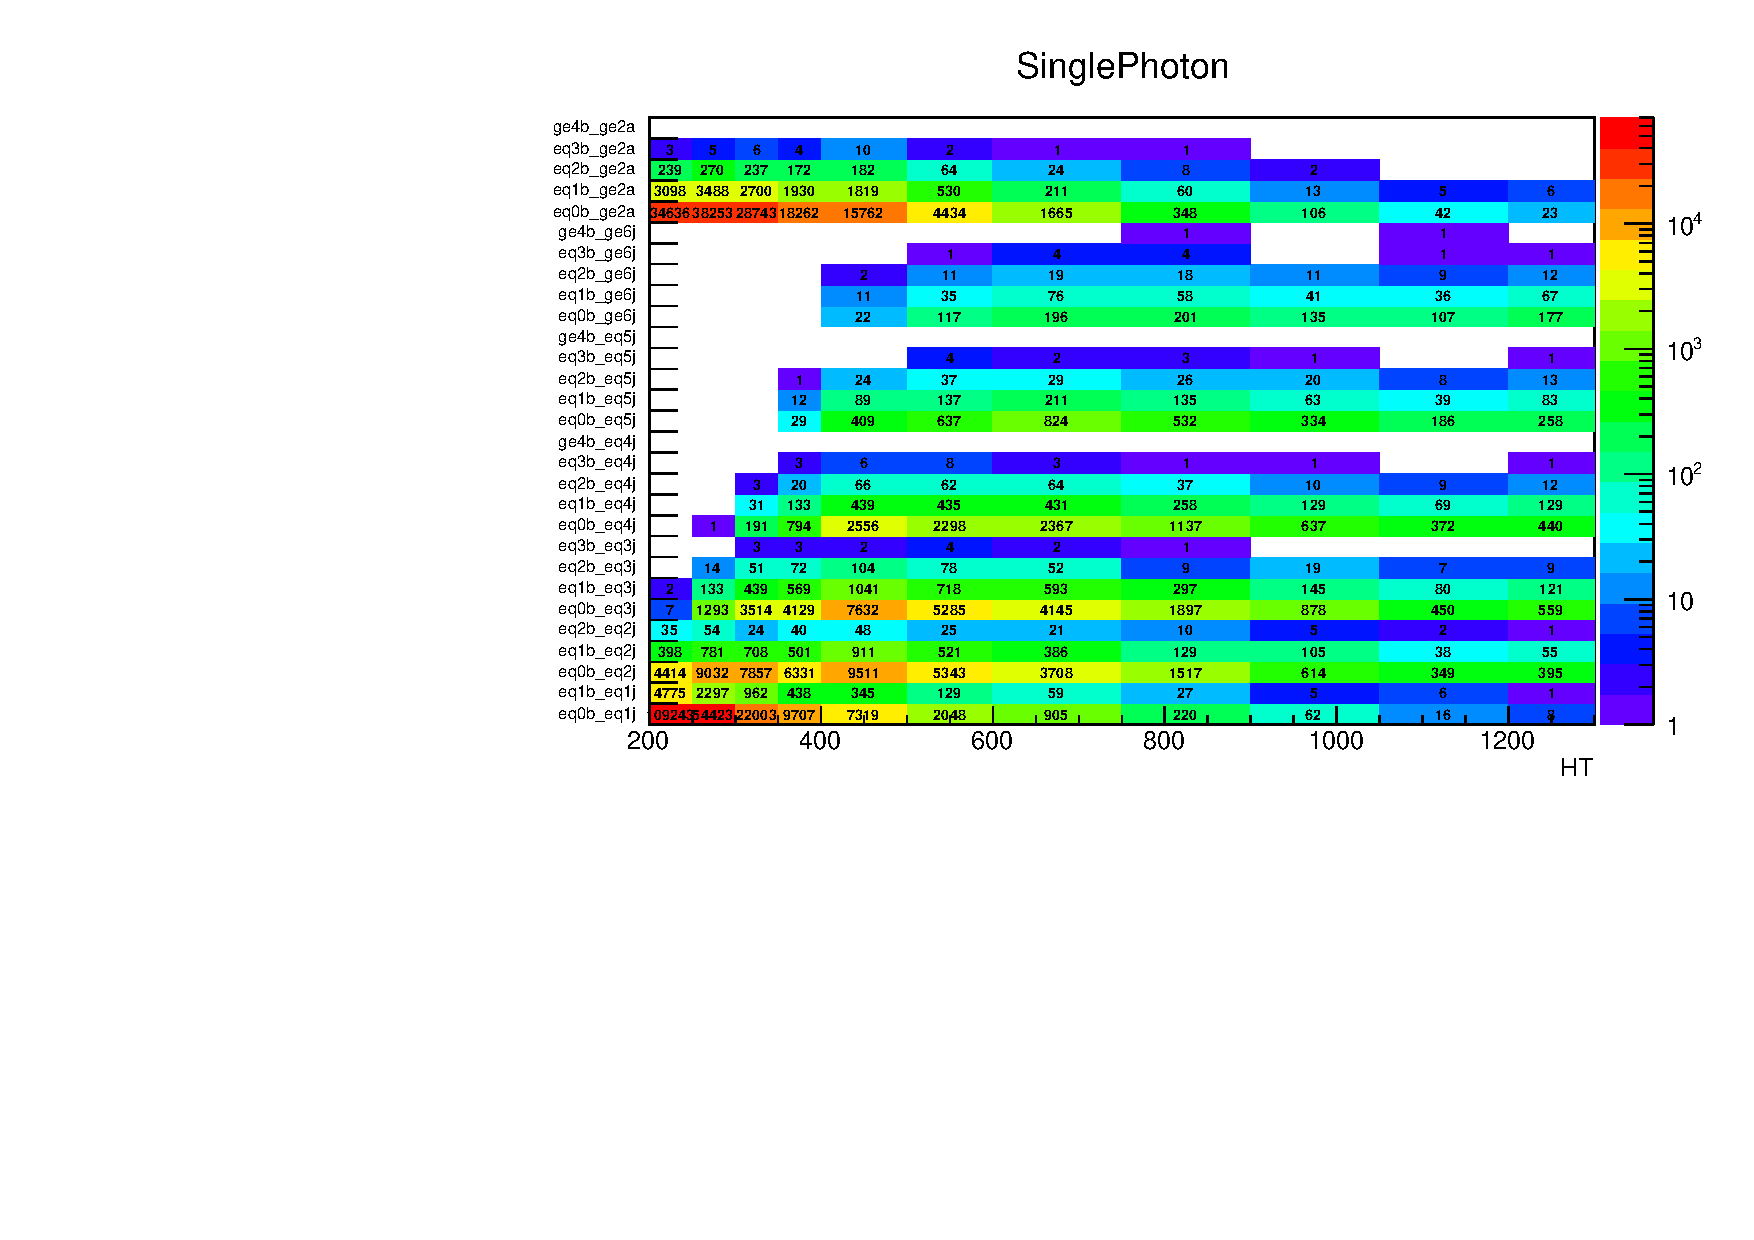
\includegraphics[width=0.6\textwidth]{figures/control_regions/SinglePhoton.pdf}}
    \caption{Event counts in data as a function of (\njet, \nb,
      \scalht) in the (Top) \mj, (Middle) \mmj, and (Bottom) \gj
      samples. Based on 35.9\fbinv. Only event counts in the \mj and
      \mmj samples are considered when determining the binning
      utilised by the analysis. The event counts for the \gj sample is
      shown for completeness.} 
    \label{fig:cr-counts}
  \end{center}
\end{figure}

\clearpage
\begin{table}[!h]
  \topcaption{Summary of the highest value of \nb used to categorise
    events as a function of \scalht [GeV] and \HTmiss [GeV] for events
    that satisfy $\njet = 1$. An identical \HTmiss binning is used for
    each \nb category, from $\nb = 0$ up to the \nb value
    indicated. The \scalht binning scheme corresponds to the
    aggregated scheme used by the signal region. The first entry per
    columnn signifies the lower bound of the first \HTmiss bin. The
    final entry per columnn signifies the lower bound of the final
    open \HTmiss bin. Gaps between entries within a column signify
    merged \HTmiss bins. An empty column signifies that the (\njet,
    \scalht) category is not used in the analysis. } 
  \label{tab:SR_binning_eq1j}
  \centering
  \begin{tabular}{lccccc}
  \hline
  \scalht [GeV] & \multicolumn{5}{c}{\HTmiss [GeV]} \\ 
  \cline{2-6}
      &      200 &      400 &      600 &      900 &     1200 \\
  \hline
  200 & 1        &          &          &          &          \\ 
  400 &          & 1        &          &          &          \\ 
  600 &          &          & 1        &          &          \\ 
  900 &          &          &          & 1        &          \\ 
  \end{tabular}
\end{table}

\begin{table}[!h]
  \topcaption{As for Table~\ref{tab:SR_binning_eq1j} with events that satisfy $\njet \geq 2 \textrm{(asymmetric topology)}$. }
  \label{tab:SR_binning_ge2a}
  \centering
  \begin{tabular}{lccccc}
  \hline
  \scalht [GeV] & \multicolumn{5}{c}{\HTmiss [GeV]} \\ 
  \cline{2-6}
      &      200 &      400 &      600 &      900 &     1200 \\
  \hline
  200 & 3        & 3        & 3        & 2        &          \\ 
  400 &          & 3        & 3        &          &          \\ 
  600 &          &          & 3        &          &          \\ 
  900 &          &          &          & 2        &          \\ 
  \end{tabular}
\end{table}

\begin{table}[!h]
  \topcaption{As for Table~\ref{tab:SR_binning_eq1j} with events that satisfy $\njet = 2$. }
  \label{tab:SR_binning_eq2j}
  \centering
  \begin{tabular}{lccccc}
  \hline
  \scalht [GeV] & \multicolumn{5}{c}{\HTmiss [GeV]} \\ 
  \cline{2-6}
      &      200 &      400 &      600 &      900 &     1200 \\
  \hline
  200 & 2        & 2        & 2        & 2        & 1        \\ 
  400 &          & 2        & 2        & 2        & 1        \\ 
  600 &          &          & 2        & 2        & 1        \\ 
  900 &          &          &          & 2        & 1        \\ 
  \end{tabular}
\end{table}

\begin{table}[!h]
  \topcaption{As for Table~\ref{tab:SR_binning_eq1j} with events that satisfy $\njet = 3$. }
  \label{tab:SR_binning_eq3j}
  \centering
  \begin{tabular}{lccccc}
  \hline
  \scalht [GeV] & \multicolumn{5}{c}{\HTmiss [GeV]} \\ 
  \cline{2-6}
      &      200 &      400 &      600 &      900 &     1200 \\
  \hline
  200 & 3        & 3        & 3        & 3        & 2        \\ 
  400 &          & 3        & 3        & 3        & 2        \\ 
  600 &          &          & 3        & 3        & 2        \\ 
  900 &          &          &          & 3        & 2        \\ 
  \end{tabular}
\end{table}

\begin{table}[!h]
  \topcaption{As for Table~\ref{tab:SR_binning_eq1j} with events that satisfy $\njet = 4$. }
  \label{tab:SR_binning_eq4j}
  \centering
  \begin{tabular}{lccccc}
  \hline
  \scalht [GeV] & \multicolumn{5}{c}{\HTmiss [GeV]} \\ 
  \cline{2-6}
      &      200 &      400 &      600 &      900 &     1200 \\
  \hline
  200 &          & 3        & 3        & 3        & 2        \\ 
  400 &          & 3        & 3        & 3        & 2        \\ 
  600 &          &          & 3        & 3        & 2        \\ 
  900 &          &          &          & 3        & 2        \\ 
  \end{tabular}
\end{table}

\begin{table}[!h]
  \topcaption{As for Table~\ref{tab:SR_binning_eq1j} with events that satisfy $\njet = 5$. }
  \label{tab:SR_binning_eq5j}
  \centering
  \begin{tabular}{lccccc}
  \hline
  \scalht [GeV] & \multicolumn{5}{c}{\HTmiss [GeV]} \\ 
  \cline{2-6}
      &      200 &      400 &      600 &      900 &     1200 \\
  \hline
  200 &          & $\geq 4$ & 3        & 3        & 2        \\ 
  400 &          & $\geq 4$ & 3        & 3        & 2        \\ 
  600 &          &          & 3        & 3        & 2        \\ 
  900 &          &          &          & 3        & 2        \\ 
  \end{tabular}
\end{table}

\begin{table}[!h]
  \topcaption{As for Table~\ref{tab:SR_binning_eq1j} with events that satisfy $\njet \geq 6$. }
  \label{tab:SR_binning_ge6j}
  \centering
  \begin{tabular}{lccccc}
  \hline
  \scalht [GeV] & \multicolumn{5}{c}{\HTmiss [GeV]} \\ 
  \cline{2-6}
      &      200 &      400 &      600 &      900 &     1200 \\
  \hline
  200 &          & $\geq 4$ & 3        & 3        & 3        \\ 
  400 &          & $\geq 4$ & 3        & 3        & 3        \\ 
  600 &          &          & 3        & 3        & 3        \\ 
  900 &          &          &          &          & 3        \\ 
  \end{tabular}
\end{table}

\clearpage 
\begin{table}[!h]
  \topcaption{Summary of the highest value of \nb used to categorise
    events as a function of \scalht [GeV] and \HTmiss [GeV] for events
    that satisfy $\njet = 1$. An identical \HTmiss binning is used for
    each \nb category, from $\nb = 0$ up to the \nb value
    indicated. The \scalht binning scheme corresponds to that used by
    the control regions. (Event yields and predictions are
    subsequently aggregated according to the binning scheme for the
    signal region.) The first entry per columnn signifies the lower
    bound of the first \HTmiss bin. The final entry per columnn
    signifies the lower bound of the final open \HTmiss bin. Gaps
    between entries within a column signify merged \HTmiss bins. An
    empty column signifies that the (\njet, \scalht) category is not
    used in the analysis. }  
  \label{tab:CR_binning_eq1j}
  \centering
  \begin{tabular}{lccccccccccc}
  \hline
  \scalht [GeV] & \multicolumn{11}{c}{\HTmiss [GeV]} \\ 
  \cline{2-12}
      &      200 &      250 &      300 &      350 &      400 &      500 &      600 &      750 &      900 &     1050 &     1200 \\
  \hline
  200 & 1        &          &          &          &          &          &          &          &          &          &          \\ 
  400 &          &          &          &          & 1        &          &          &          &          &          &          \\ 
  600 &          &          &          &          &          &          & 1        &          &          &          &          \\ 
  900 &          &          &          &          &          &          &          &          & 1        &          &          \\ 
  \end{tabular}
\end{table}

\begin{table}[!h]
  \topcaption{As for Table~\ref{tab:CR_binning_eq1j} with events that satisfy $\njet \geq 2 \textrm{(asymmetric topology)}$. }
  \label{tab:CR_binning_ge2a}
  \centering
  \begin{tabular}{lccccccccccc}
  \hline
  \scalht [GeV] & \multicolumn{11}{c}{\HTmiss [GeV]} \\ 
  \cline{2-12}
      &      200 &      250 &      300 &      350 &      400 &      500 &      600 &      750 &      900 &     1050 &     1200 \\
  \hline
  200 & 3        & 3        & 3        & 3        & 3        & 3        & 3        & 2        & 2        &          &          \\ 
  400 &          &          &          &          & 3        & 3        & 3        &          &          &          &          \\ 
  600 &          &          &          &          &          &          & 3        &          &          &          &          \\ 
  900 &          &          &          &          &          &          &          &          & 2        &          &          \\ 
  \end{tabular}
\end{table}

\begin{table}[!h]
  \topcaption{As for Table~\ref{tab:CR_binning_eq1j} with events that satisfy $\njet = 2$. }
  \label{tab:CR_binning_eq2j}
  \centering
  \begin{tabular}{lccccccccccc}
  \hline
  \scalht [GeV] & \multicolumn{11}{c}{\HTmiss [GeV]} \\ 
  \cline{2-12}
      &      200 &      250 &      300 &      350 &      400 &      500 &      600 &      750 &      900 &     1050 &     1200 \\
  \hline
  200 & 2        & 2        & 2        & 2        & 2        & 2        & 2        & 2        & 2        & 1        & 1        \\ 
  400 &          &          &          &          & 2        & 2        & 2        & 2        & 2        & 1        & 1        \\ 
  600 &          &          &          &          &          &          & 2        & 2        & 2        & 1        & 1        \\ 
  900 &          &          &          &          &          &          &          &          & 2        & 1        & 1        \\ 
  \end{tabular}
\end{table}

\begin{table}[!h]
  \topcaption{As for Table~\ref{tab:CR_binning_eq1j} with events that satisfy $\njet = 3$. }
  \label{tab:CR_binning_eq3j}
  \centering
  \begin{tabular}{lccccccccccc}
  \hline
  \scalht [GeV] & \multicolumn{11}{c}{\HTmiss [GeV]} \\ 
  \cline{2-12}
      &      200 &      250 &      300 &      350 &      400 &      500 &      600 &      750 &      900 &     1050 &     1200 \\
  \hline
  200 & 3        & 3        & 3        & 3        & 3        & 3        & 3        & 3        & 3        & 2        & 2        \\ 
  400 &          &          &          &          & 3        & 3        & 3        & 3        & 3        & 2        & 2        \\ 
  600 &          &          &          &          &          &          & 3        & 3        & 3        & 2        & 2        \\ 
  900 &          &          &          &          &          &          &          &          & 3        & 2        & 2        \\ 
  \end{tabular}
\end{table}

\begin{table}[!h]
  \topcaption{As for Table~\ref{tab:CR_binning_eq1j} with events that satisfy $\njet = 4$. }
  \label{tab:CR_binning_eq4j}
  \centering
  \begin{tabular}{lccccccccccc}
  \hline
  \scalht [GeV] & \multicolumn{11}{c}{\HTmiss [GeV]} \\ 
  \cline{2-12}
      &      200 &      250 &      300 &      350 &      400 &      500 &      600 &      750 &      900 &     1050 &     1200 \\
  \hline
  200 &          &          &          &          & 3        & 3        & 3        & 3        & 3        & 2        & 2        \\ 
  400 &          &          &          &          & 3        & 3        & 3        & 3        & 3        & 2        & 2        \\ 
  600 &          &          &          &          &          &          & 3        & 3        & 3        & 2        & 2        \\ 
  900 &          &          &          &          &          &          &          &          & 3        & 2        & 2        \\ 
  \end{tabular}
\end{table}

\begin{table}[!h]
  \topcaption{As for Table~\ref{tab:CR_binning_eq1j} with events that satisfy $\njet = 5$. }
  \label{tab:CR_binning_eq5j}
  \centering
  \begin{tabular}{lccccccccccc}
  \hline
  \scalht [GeV] & \multicolumn{11}{c}{\HTmiss [GeV]} \\ 
  \cline{2-12}
      &      200 &      250 &      300 &      350 &      400 &      500 &      600 &      750 &      900 &     1050 &     1200 \\
  \hline
  200 &          &          &          &          & $\geq 4$ & 3        & 3        & 3        & 3        & 2        & 2        \\ 
  400 &          &          &          &          & $\geq 4$ & 3        & 3        & 3        & 3        & 2        & 2        \\ 
  600 &          &          &          &          &          &          & 3        & 3        & 3        & 2        & 2        \\ 
  900 &          &          &          &          &          &          &          &          &          & 2        & 2        \\ 
  \end{tabular}
\end{table}

\begin{table}[!h]
  \topcaption{As for Table~\ref{tab:CR_binning_eq1j} with events that satisfy $\njet \geq 6$. }
  \label{tab:CR_binning_ge6j}
  \centering
  \begin{tabular}{lccccccccccc}
  \hline
  \scalht [GeV] & \multicolumn{11}{c}{\HTmiss [GeV]} \\ 
  \cline{2-12}
      &      200 &      250 &      300 &      350 &      400 &      500 &      600 &      750 &      900 &     1050 &     1200 \\
  \hline
  200 &          &          &          &          & $\geq 4$ & 3        & 3        & 3        & 3        & 3        & 3        \\ 
  400 &          &          &          &          &          & 3        & 3        & 3        & 3        & 3        & 3        \\ 
  600 &          &          &          &          &          &          &          & 3        & 3        &          & 3        \\ 
  900 &          &          &          &          &          &          &          &          &          &          & 3        \\ 
  \end{tabular}
\end{table}

